\begin{figure}[H]
	\center

	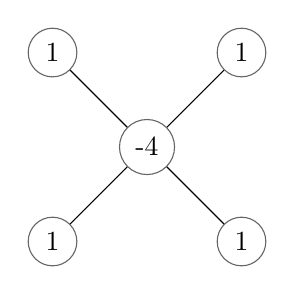
\begin{tikzpicture}

	\def \xone{0};
	\def \yone{0};
	\def \h{1.2}	

	\coordinate (M) at (\xone ,\yone);
	\coordinate (LU) at (\xone-\h ,\yone-\h);
	\coordinate (RU) at (\xone+\h ,\yone-\h);
	\coordinate (LO) at (\xone-\h ,\yone+\h);
	\coordinate (RO) at (\xone+\h ,\yone+\h);
	\draw (LU) -- (RO);
	\draw (RU) -- (LO);

	%draw nodes
	\node[circle,draw=black!60, fill=white!40] at (M) {-4};
	\node[circle,draw=black!60, fill=white!40] at (LO) {1};
	\node[circle,draw=black!60, fill=white!40] at (RO) {1};
	\node[circle,draw=black!60, fill=white!40] at (LU) {1};
	\node[circle,draw=black!60, fill=white!40] at (RU) {1};

		
	\end{tikzpicture}
\caption{rotated 5-point stencil}
\label{five_point_rot}
	
\end{figure}
